\chapter{Introduction and Literature Review}
\label{ch:introduction}

The usual approach
to investigating the effect of domain shape
on solutions to a boundary value problem (BVP)
is simply to solve the BVP in various domains.
For any given domain shape, one seeks solutions
to the associated partial differential equation (PDE) in the interior
which also satisfy the prescribed boundary conditions on the boundary.
In linear problems possessing sufficient symmetry,
the superposition principle
together with separation of variables or integral transforms
would typically allow us to complete this task,
but in nonlinear problems,
exact solutions are rare and often only available for simple geometries.
From a numerical viewpoint
it can also be computationally expensive
to consider many different domain shapes,
since the BVP must be solved from scratch for each new domain.

An alternative strategy is to
consider the BVP in reverse:
given a solution to the PDE\@, are there new boundaries
which also satisfy the prescribed boundary conditions?
If so, it is conceivable that these new boundaries may be used
to construct new domains
which admit the same solution to the given BVP\@.
Such an approach has been employed in an \adhoc{} fashion
by Anderssen~\etal~\cite{anderssen-1969-ion-uptake-growing-roots}
to numerically determine the profile of a growing root
and by McNabb~\etal~\cite{mcnabb-1991-theoretical-derivation-freezing-times}
to estimate finite measures of cooling time in ellipsoids.
The first systematic investigation of this
reverse strategy for flux boundary conditions,
known as \term{boundary tracing},
was carried out by
Anderson~\etal~\cite{anderson-2007-boundary-tracing-i-theory}
with applications to the \laplaceyoung{} equation
of capillarity~\cite{anderson-2006-exact-solutions-laplace-young}
and other PDEs, including the Helmholtz,
constant mean curvature, and
Poisson equations~\cite{anderson-2007-boundary-tracing-ii-applications}.

Over a decade has since passed
with little further work in the area,
and the aim of this thesis is to
continue the application of boundary tracing
to physically significant contexts;
its use in a thermal radiation problem is explored
and the work on capillarity is extended.
We begin with a brief introduction to boundary tracing
and a review of the relevant known results
in thermal radiation and capillarity.

\section{Boundary tracing}
\label{sec:introduction.tracing}

This section provides a quick overview of
the theory of \term{boundary tracing},
which is well described by
Anderson~\etal~\cite{anderson-2007-boundary-tracing-i-theory}.
A more detailed description can be found in
Anderson's thesis~\cite{anderson-2002-thesis-boundary-tracing-pdes}.

Consider a BVP\@, consisting of
a PDE in some two-dimensional domain~$\Omega$
together with the boundary condition
\begin{important}{equation}
  \normalvec \dotp \del T = F \roundbr[\bulkysize]{x, y, T, \norm{\del T}}
  \label{eq:flux-boundary-condition}
\end{important}
on its boundary~$\pd\Omega$,
where $\normalvec$~is the outward-pointing unit normal
and $F$~is a given \term{flux function}.
Whereas the usual goal is
to determine the solution~$T$ for a given domain~$\Omega$,
the aim of boundary tracing is
to seek~$\Omega$ for a given~$T$.
Specifically, we take any known solution~$T = T (x, y)$ to the PDE
and seek \term{traced boundaries}, which are curves
along which the flux condition~(\ref{eq:flux-boundary-condition}) holds.
Once the traced boundaries have been found,
we may use them to construct new domains
for which the solution to the BVP is also~$T$.

\begin{figure}
  \newcommand*{\subfigurewidth}{0.325\textwidth}
  \centering
  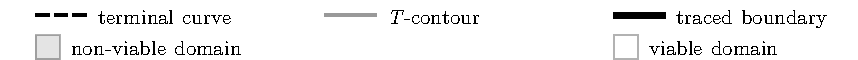
\includegraphics[width=\textwidth]{terminal-legend}
  \begin{subfigure}{\subfigurewidth}
    \centredfigurecontent{terminal-ordinary}{Ordinary}
  \end{subfigure}
  \hfill
  \begin{subfigure}{\subfigurewidth}
    \centredfigurecontent{terminal-critical_hyperbolic}{Critical: hyperbolic}
  \end{subfigure}
  \hfill
  \begin{subfigure}{\subfigurewidth}
    \centredfigurecontent{terminal-critical_elliptic}{Critical: elliptic}
  \end{subfigure}
  \caption{
    Terminal curve, local $T$-contour, and traced boundaries
    through a terminal point.
  }
  \label{fig:terminal}
\end{figure}

The flux condition~(\ref{eq:flux-boundary-condition})
is best understood as a geometric constraint:
at any point~$(x, y)$ in the domain of~$T$,
it determines the possible local orientations for~$\normalvec$,
and therefore, the possible local orientations
of the sought-after traced boundaries
(which have normal~$\normalvec$).
With $\theta$ denoting the angle between~$\normalvec$ and~$\del T$,
the boundary condition~(\ref{eq:flux-boundary-condition}) may be rewritten as
\begin{equation}
  \cos\theta = \frac{F}{\norm{\del T}},
  \label{eq:flux-boundary-condition-cosine}
\end{equation}
and there are three cases at any given point:
\begin{enumerate}
  \item
    If~$\norm{\del T} > \abs{F}$,
    then~(\ref{eq:flux-boundary-condition-cosine})
    has a conjugate pair of solutions in~$\theta$.
    There are two choices for~$\normalvec$
    (symmetric about~$\del T$)
    corresponding to two possible local orientations
    for the traced boundaries,
    which cross the local $T$-contour at an angle.
  \item
    If~$\norm{\del T} = \abs{F}$,
    then $\normalvec$~is either parallel~($\theta = 0$)
    or antiparallel~($\theta = \pi$) to~$\del T$,
    corresponding to traced boundaries which are tangential
    to the local $T$-contour.
  \item
    If~$\norm{\del T} < \abs{F}$,
    then the right hand side of~(\ref{eq:flux-boundary-condition-cosine})
    exceeds unity in magnitude,
    and there are no solutions in~$\theta$,
    i.e.~traced boundaries do not exist.
\end{enumerate}
This naturally suggests a partitioning of
the domain of the known solution~$T$ into
the \term{viable domain}~$\norm{\del T} \ge \abs{F}$,
in which there are two possible branches of traced boundaries,
and the \term{non-viable domain}~$\norm{\del T} < \abs{F}$,
in which traced boundaries cannot exist.
The border between these two regions is
the \term{terminal curve}~$\norm{\del T} = \abs{F}$,
along which traced boundaries are tangential to the local $T$-contour.

A point along the terminal curve is called a \term{terminal point},
and is one of the following:
\begin{enumerate}
  \item
    An \term{ordinary} terminal point
    (Figure~\ref{fig:terminal-ordinary}):
    the local $T$-contour crosses the terminal curve at a non-zero angle.
    The traced boundaries (which are tangential to the local $T$-contour)
    terminate in a cusp at the terminal point,
    for they cannot enter the non-viable domain.
  \item
    A \term{critical} terminal point:
    the local $T$-contour touches the terminal curve tangentially.
    This results in one of the following:
    \begin{enumerate}
      \item
        The \term{hyperbolic} case
        (Figure~\ref{fig:terminal-critical_hyperbolic}):
        the $T$-contour lies toward the viable side of the terminal curve.
        Two smooth traced boundaries pass through the terminal point,
        at which the traced boundaries,
        the local $T$-contour and the terminal curve
        all touch.
      \item
        The \term{elliptic} case
        (Figure~\ref{fig:terminal-critical_elliptic}):
        the $T$-contour lies toward the non-viable side of the terminal curve,
        and no smooth traced boundaries pass through the terminal point.
      \item
        The \term{degenerate} case:
        the $T$-contour and the entire terminal curve
        are in fact the same curve.
        Thus the terminal curve consists solely of critical terminal points,
        and is therefore called a \term{critical terminal curve}.
        This curve is itself a traced boundary,
        unto which other traced boundaries attach smoothly.
    \end{enumerate}
    The degenerate case occurs
    when the known solution~$T$ possesses sufficient symmetry.
    Anderson~\etal~\cite{anderson-2007-boundary-tracing-i-theory}
    note that they have not encountered any case
    where a non-discrete proper subset of the terminal curve
    coincides with a $T$-contour;
    neither will we encounter such a case in this thesis.
\end{enumerate}

To determine the sought-after traced boundaries,
simply choose an appropriate coordinate system and parametrisation,
rewrite the flux condition~(\ref{eq:flux-boundary-condition})
as an ordinary differential equation (ODE) for the traced boundaries,
and integrate.
By patching together the traced boundaries which result,
new domains may be constructed
which also admit the solution~$T$ to the given BVP\@.
The only restriction on the manner of patching
is that the boundary normal~$\normalvec$ have consistent orientation
with respect to the flux condition~(\ref{eq:flux-boundary-condition}),
and it is here that
the distinction between ordinary and critical terminal points
becomes important.
Generally speaking we must avoid ordinary terminal points;
the cusp formed by the two traced boundaries
will not have consistent boundary orientation,
except possibly for vanishing or discontinuous~$F$.

Anderson~\etal~\cite{anderson-2007-boundary-tracing-i-theory}
have also derived results for the curvature of traced boundaries
and given a very neat analysis of boundary tracing
by mapping the curves onto the manifold~$z^2 = (\del T)^2 - F^2$.
While both of these are of utmost theoretical importance
(indeed a proper understanding of and classification system for
critical terminal points was a result of the manifold analysis),
we will not need them for the boundary tracing work in this thesis.

To summarise, boundary tracing is a method in which
a known solution to a PDE is used
to generate new domains which admit the same solution
to the associated BVP
with flux boundary condition~(\ref{eq:flux-boundary-condition}).
It is fitting to conclude this overview with the observation that
boundary tracing is \emph{not} a perturbative method.
No approximation is required
to convert the flux condition~(\ref{eq:flux-boundary-condition})
into an ODE for the traced boundaries,
and although numerical procedures may be required
to do the subsequent integration,
the underlying theory is exact.

\section{Thermal radiation}
\label{sec:introduction.radiation}

In this section
we briefly review the literature for
a simple conduction--radiation problem,
to which the application of boundary tracing is well suited.

In outer space,
thermal radiation is the primary means of disposing of waste heat.
An archetypal steady-state problem consists of
determining the temperature profile~$T$ of a conducting object~$\Omega$,
with heat generated internally or towards one end
and expelled into vacuum via radiation from its surface.

Assuming that the object is homogeneous and isotropic,
with temperature-independent thermal properties,
the steady conduction within~$\Omega$
is simply described by Laplace's equation
\begin{equation}
  \del^2 T = 0,
  \label{eq:laplace-steady-conduction}
\end{equation}
but on the portion of its surface~$\pd \Omega$
(assumed grey and diffuse) where radiation occurs,
the \stefanboltz{} law implies that
\begin{equation}
  \normalvec \dotp \del T = - c T^4,
  \label{eq:radiation-boundary-condition}
\end{equation}
where
\begin{equation}
  c = \frac{\emiss \stefan}{\conduc},
  \label{eq:radiation-constant}
\end{equation}
with $\conduc$~being the conductivity of the object,
$\emiss$~the emissivity of its surface,
and $\stefan = \SI{5.67e-8}{\watt \per\metre\squared \per\kelvin\tothe{4}}$~%
the \stefanboltz{} constant~%
\cite{tiesinga-2019-2018-codata-recommended-constants}.

This boundary value problem is not straightforward
even in two dimensions,
due to the nonlinearity of
the radiation condition~(\ref{eq:radiation-boundary-condition}).
The usual treatment in the literature has been to consider thin geometries
for which the problem is effectively one-dimensional,
so that the conduction~(\ref{eq:laplace-steady-conduction})
and the radiation~(\ref{eq:radiation-boundary-condition})
may be lumped into a single ODE of the form
\begin{equation}
  \textq{derivatives of~$T$} - c T^4 = 0.
  \label{eq:conduction-radiation-lumped}
\end{equation}
Indeed this has been the approach taken in the analytical investigations of
Liu~\cite{liu-1960-minimum-rectangular-radiating-fins},
Wilkins~\cite{
  wilkins-1960-minumum-mass-fins-radiation,
  wilkins-1961-minimum-mass-fins-thickness,
  wilkins-1962-minimum-mass-fins-gradients,
  wilkins-1974-optimum-shapes-convection-radiation
},
and
Shouman~\cite{shouman-1968-exact-radiation-convection-fin},
and in numerical work by
Chambers \&~Somers~\cite{chambers-1959-radiation-fin-efficiency-circular},
Lieblein~\cite{lieblein-1959-radiant-fin-constant-thickness},
Bartas \&~Sellers~\cite{bartas-1960-radiation-fin-effectiveness},
and
Keller \&~Holdredge~\cite{keller-1970-radiation-annular-fins-trapezoidal}.
While such a simplification is an appropriate choice
for the study of thin, heat-rejecting fins on spacecraft
(where thinness and minimisation of weight are desirable),
it has also arguably been a necessity
for making the BVP~(\ref{eq:laplace-steady-conduction})
and~(\ref{eq:radiation-boundary-condition}) analytically tractable;
there appears to be no analytical treatment
of a conduction--radiation problem
in which the nonlinearity appears as a proper boundary term
in the flux condition~(\ref{eq:radiation-boundary-condition}),
rather than as a volumetric term in an ODE
of the form~(\ref{eq:conduction-radiation-lumped}).

Given the relative abundance of known solutions
to Laplace's equation~(\ref{eq:laplace-steady-conduction}),
and the limited amount of progress which can be made
using conventional techniques
for the nonlinear boundary condition~(\ref{eq:radiation-boundary-condition}),
boundary tracing is a most suitable method
for tackling the BVP~(\ref{eq:laplace-steady-conduction})
and~(\ref{eq:radiation-boundary-condition}),
being an analytical approach
which does not require reducing the problem to one dimension.

\section{Capillarity}
\label{sec:introduction.capillarity}

In this section the capillary wedge problem is introduced,
and we review both boundary tracing and conventional approaches
in the literature.

If a liquid is poured into a vertically-walled container,
the liquid surface will not be level at equilibrium,
but will instead be curved near the container walls
(e.g.~the meniscus formed by water in a test tube).
The physical effect is that of surface tension,
a balance between the forces of cohesion (liquid--liquid attraction),
adhesion (liquid--wall attraction), and gravity.

One practical application
where surface tension plays an important role
is industrial dip-coating.
In a problem described by
King~\etal~\cite{king-1999-laplace-young-near-corner},
a rectangular prism is dipped into a liquid to coat its bottom half;
the end result is a coating layer
that exhibits undesirable arching near the corners of the prism
(Figure~X). % TODO
Fowkes \&~Hood~\cite{fowkes-1998-surface-tension-effects-wedge}
have suggested corner rounding as a practical means of reducing arching,
but note that numerical methods are likely required
to analyse the rounded-corner scenario.
The behaviour of capillary surfaces near both sharp and rounded corners
is therefore of considerable interest.

\section{Thesis overview}
